\label{modbus_kapitel}
Die offizielle Definition des \gls{modbus} Protokolls von der \gls{modbus} Organization \cite[vgl.][]{Modbus_Organization_AP:2012} lautet:
\begin{quotation}
	\noindent\emph{\enquote{MODBUS is an application layer messaging protocol, positioned at level 7 of the OSI model, which provides client/server communication between devices connected on different types of buses or networks.}}
\end{quotation}

\noindent Der \gls{modbus} Standard definiert ein Application Layer Kommunikations Protokoll, das sich auf Schicht 7 des \gls{osi} Modells befindet. Es bietet \gls{client}/\gls{server} Kommunikation zwischen Geräten, die auf verschiedenen Bussen oder Netzwerken angeschlossen sind.

Das \gls{modbus} Protokoll wurde 1979 von der Firma Gould-Modicon entwickelt. Besonders wird das Protokoll in Mess- und Regelsystemen eingesetzt, da es speziell für die Kommunikation mit speicherprogrammierbaren Steuerungen entwickelt wurde. Das \gls{modbus} Protokoll ist ein Industriestandard. Es bietet einen universellen Übertragungsweg, ganz egal welches Übertragungsmedium genutzt wird. Es funktioniert sowohl über ein serielles Bussystem, als auch über eine Netzwerkverbindung. Außerdem können mit sogenannten Protokollumsetzern Geräte mit serieller Kommunikation in ein Netzwerksystem eingebettet werden. Durch den Einsatz von Paritätsprüfungen und Checksummen gewährleistet das Protokoll eine zuverlässige Übertragung. \cite[vgl.][]{KUNBUS_GmbH:o.J., kvm-concepts_GmbH:2022}


Die folgende theoretische Beschäftigung mit dem \gls{modbus} Protokoll bezieht sich wenn nicht anders angegeben auf die offiziellen \gls{modbus} Dokumentationen. \cite[vgl.][]{Modbus_Organization_AP:2012, Modbus_Organization_SL:2012}

Da das \gls{modbus} Protokoll nur Layer 7 des \gls{osi} Modells definiert, kann es in verschiedenen Übertragungssystemen implementiert werden:
\begin{itemize}
	\item \textbf{\gls{modbus} \acs{tcp}:} Die Geräte sind an einem Netzwerk angeschlossen und kommunizieren via \acs{tcp}/IP.
	\item \textbf{\gls{modbus} Serial Line:} Die Geräte sind hier an einem seriellen Bus angeschlossen. Dabei gibt es zwei Übertragungsarten, nämlich \acs{rtu} und \acs{ascii}. Genauere Beschreibungen der beiden Übertragungsarten finden sich später in diesem Kapitel.
	\item \textbf{\gls{modbus} Plus:} Funktioniert mittels eines Tokens. Jeweils das Gerät, welches den Token aktuell besitzt, ist der \gls{client} und kann die Kommunikation mit den anderen Geräten initialisieren. Wenn der derzeitige \gls{client} keine Nachrichten mehr senden muss, gibt er den Token an das nächste Gerät weiter. \cite[vgl.][]{Rinaldi:2016}
\end{itemize}

Folgende Grafik (Siehe Abb.~\ref{fig:modbus_stack}) illustriert horizontal die unterschiedlichen Übertragungssysteme und vertikal welche Schichten von darunterliegenden Protokollen und Technologien besetzt werden.
\begin{figure}[H]
	\centering
	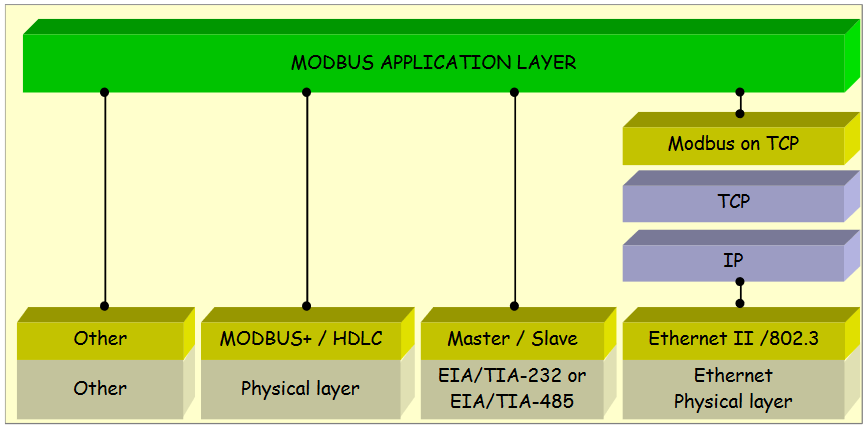
\includegraphics[width=1.0\linewidth]{Bilder/Modbus_layers}
	\caption[\gls{modbus} Stack (Quelle: \url{https://modbus.org/docs/Modbus_Application_Protocol_V1_1b3.pdf}, Zugriff am 25.02.2024)]{\gls{modbus} Stack (Quelle: \url{https://modbus.org/docs/Modbus_Application_Protocol_V1_1b3.pdf})}
	\label{fig:modbus_stack}
\end{figure}

\subsection{Funktionsweise} \label{modbus_funktionsweise}
\gls{modbus} verwendet das \gls{client}/\gls{server} System. In einem Bussystem kann es nur einen \gls{client} geben. Es können jedoch beliebig viele \gls{server} am Bus angeschlossen werden. Der \gls{client} kann die Kommunikation mit den einzelnen \gls{server}n initialisieren. Er kann ihnen Daten senden und von ihnen Daten anfordern. Ein \gls{server} hingegen kann keine Kommunikation beginnen, sondern lediglich auf Anfrage des \gls{client}s handeln.

Jeder \gls{server} am Bus hat eine einzigartige Adresse. Die Adressen können Werte von 0 bis 255 einnehmen (siehe Tab.~\ref{tab:modbus_adressen} für die Einteilung). 
\begin{table}[H]
	\caption{\gls{modbus} Adressen Einteilung \label{tab:modbus_adressen}}
	\begin{tabularx}{\textwidth}{@{}c|c|X@{}}
		\toprule
		\textbf{Adressen} & \textbf{Bezeichnung} & \textbf{Beschreibung} \\
		\midrule
		0 & Broadcast & Hiermit sendet der \gls{client} eine Anfrage an alle \gls{server} am Bus. Diese senden keine Antwort zurück. \\
		1 - 247 & \gls{server} & Der \gls{client} kann damit einzelne \gls{server} ansprechen. Diese senden dem \gls{client} eine Antwort zurück. \\
		248 - 255 & Anderweitig reserviert & \\
		\bottomrule
	\end{tabularx}
\end{table}